\documentclass[a4paper]{article}

%% Language and font encodings
\usepackage[french]{babel}
\usepackage[utf8]{inputenc}
\usepackage[T1]{fontenc}

\usepackage{float}

\setlength{\parindent}{1em}
%\setlength{\parskip}{1ex plus 0.5ex minus 0.2ex}
\newcommand{\hsp}{\hspace{20pt}}
\newcommand{\HRule}{\rule{\linewidth}{0.5mm}}

\usepackage{algorithm}
\usepackage[noend]{algpseudocode}
\algnewcommand{\algorithmicand}{\textbf{ and }}
\algnewcommand{\algorithmicor}{\textbf{ or }}
\algnewcommand{\OR}{\algorithmicor}
\algnewcommand{\AND}{\algorithmicand}
\algnewcommand\algorithmicforeach{\textbf{for each}}
\algdef{S}[FOR]{ForEach}[1]{\algorithmicforeach\ #1\ \algorithmicdo}
\newcommand{\myfrac}[2]{\frac{\displaystyle {#1}}{\displaystyle {#2}}}

%% Sets page size and margins
\usepackage[a4paper,top=3cm,bottom=2cm,left=3cm,right=3cm,marginparwidth=1.75cm]{geometry}

%% Useful packages
\usepackage{amsmath}
\usepackage{amssymb}
\usepackage{graphicx}
\usepackage{subcaption}
\usepackage[colorinlistoftodos]{todonotes}
\usepackage[colorlinks=true, allcolors=blue]{hyperref}
\usepackage{graphicx}

\usepackage{enumitem}
\setitemize{label=\textbullet, font=\small}

%% equations
\usepackage{amsthm}
\usepackage[retainorgcmds]{IEEEtrantools}

%% theorem and proposition
\newtheorem{prop}{Proposition}
\newtheorem*{prop*}{Proposition}
\newtheorem{thm}{Théorème}

\newenvironment{myproof}[1][\proofname]{\proof[#1]\mbox{}\\*}{\endproof}

%% references shortcuts (Arthur) 
\usepackage{suffix}
\renewcommand{\eqref}[1]{équation~\ref{#1}}
\newcommand{\algoref}[1]{algorithme~\ref{#1}}
\newcommand{\figref}[1]{figure~\ref{#1}}
\newcommand{\tabref}[1]{tableau~\ref{#1}}
\newcommand{\secref}[1]{section~\ref{#1}}
\newcommand{\probref}[1]{problème~\ref{#1}}
\newcommand{\propref}[1]{proposition~\ref{#1}}
\newcommand{\theoremref}[1]{théorème~\ref{#1}}
\newcommand{\chapref}[1]{chapitre~\ref{#1}}
\WithSuffix\newcommand\algoref*[1]{algorithme~\ref{#1} p.~\pageref{#1}}
\WithSuffix\newcommand\figref*[1]{figure~\ref{#1} p.~\pageref{#1}}
\WithSuffix\newcommand\eqref*[1]{équation~\ref{#1} p.~\pageref{#1}}
\WithSuffix\newcommand\tabref*[1]{tableau~\ref{#1} p.~\pageref{#1}}
\WithSuffix\newcommand\secref*[1]{section~\ref{#1} p.~\pageref{#1}}
\WithSuffix\newcommand\probref*[1]{problème~\ref{#1} p.~\pageref{#1}}
\WithSuffix\newcommand\propref*[1]{proposition~\ref{#1} p.~\pageref{#1}}
\WithSuffix\newcommand\chapref*[1]{chapitre~\ref{#1} p.~\pageref{#1}}

\usepackage[backend=biber,uniquename=init,giveninits=true,
             %% "et al" pour > deux auteurs, & pour exactement 2
             uniquelist=false,maxcitenames=2,mincitenames=1,maxbibnames=99,
             isbn=false,url=false,doi=false,bibstyle=numeric
]{biblatex}
\addbibresource{references.bib}

\begin{document}

\begin{titlepage}
  \begin{center}

      \makebox[0.5\textwidth][r]{%
        
\includegraphics[width=0.33\textwidth]{images/sorbonne.png}%
    }%

      \vspace{4cm}
    % Title
    \HRule \\[0.4cm]
    { \huge \bfseries BIMA\\[0.4cm] }

      \textsc{\LARGE Mini rapport 1}\\[0.4cm]

    \HRule \\[0.8cm]
    %\HRule \\[2cm]
    %\includegraphics[scale=0.2]{images/.JPG}
    %\\[2cm]

    % Author and supervisor
    \begin{minipage}{0.4\textwidth}
      \begin{flushleft} \large
        Kim-Anh Laura \textsc{Nguyen}\\
        \large
        Arij \textsc{Riabi}\\
        M1 DAC\\
        Promo 2018-2019 \\
      \end{flushleft}
    \end{minipage}
    \begin{minipage}{0.5\textwidth}
      \begin{flushright} \large
        \emph{Enseignant :} Dominique \textsc{Béréziat}\\
      \end{flushright}
    \end{minipage}

      \vspace{2cm}

  \end{center}
  %\end{sffamily}
\end{titlepage}
%\maketitle

\newpage

\section*{Échantillonnage des signaux 2D}

En considérant une grille carrée, l'échantillonnage idéal d'un signal
2D est modélisé de la manière suivante :

\begin{equation}
    x_e(t,u) = x(t,u) \cdot e(t,u)
\label{eq:sig-e}
\end{equation}

où $e(t,u) = \sum_{k=-\infty}^{+\infty}\sum_{l=-\infty}^{+\infty}
\delta(t-kT_e,u-lT_e)$.\\

Le spectre du signal échantillonné s'écrit :

\begin{equation}
    X_e(f,g) =
    \frac{1}{T_{e}^2}\sum_{k=-\infty}^{+\infty}\sum_{l=-\infty}^{+\infty}
    X(f-kf_e,g-lf_e)
\label{eq:spectre-e}
\end{equation}

\section{Aliasing et fenêtrage pour des signaux 2D}

\subsection*{Question 1}

La \figref{img:sin1} représente l'image produite par $s_{\theta}(t,u)$,
avec $A=10$, $\theta=45^\circ$, $L=512$, $T_0=64$, et $T_e=1$.

\begin{figure}[H]
	\center 
	
\includegraphics[width=0.6\textwidth]{images/sin1.png}
    \caption{$s_{\theta}(t,u)$,
avec $A=10$, $\theta=45^\circ$, $L=512$, $T_0=64$, et $T_e=1$
}
    \label{img:sin1}
\end{figure}

\subsection*{Question 2}

La transformée de Fourier du signal $s_{\theta}(t,u)$ est :

\begin{IEEEeqnarray*}{rCl"s}
    S(f,g) &=& TF[s_{\theta}(t,u)](f,g) \\
           &=& \frac{A}{2} [\delta(f-f_0 \cos \theta) \delta(g-f_0 \sin \theta)
           + \delta(f + f_0 \cos \theta) \delta(g + f_0 \sin \theta)]\\
\end{IEEEeqnarray*}

On a alors $f^{max}_t = f_0 \cos \theta$ et $f^{max}_u = f_0 \sin \theta$.\\

Pour $T_0 = 64$ et $\theta = 45 ^\circ$, on a donc $f^{max}_t = \frac{1}{64}
\cos(45) = 0.0082$ et $f^{max}_u = \frac{1}{64} \sin(45) = 0.0133$. Donc $f_m =
max(f^{max}_t, f^{max}_u) = f^{max}_u = 0.0133$. \\

Soit $f_{max}$ la fréquence maximale du signal analogique $x_a(t)$ et $f_e$ la
fréquence du signal échantillonné $x_e(t)$. D'après le théorème de
Nyquist-Shannon, il n'y a pas de perte d'information entre $x_a(t)$ et $x_e(t)$
si :

$$ f_e \geq 2f_{max}$$

$f_m$ est donc la fréquence qui déterminera la fréquence d'échantillonnage
limite. \\

\textbf{(2a)} On échantillone $s_{\theta}(t,u)$ avec les mêmes paramètres que
précédemment et $f_e = 16 \cdot f_m = 16 \cdot 0.0133$. Le résultat est
représenté dans la \figref{img:sin16}.

\begin{figure}[H]
	\center 
	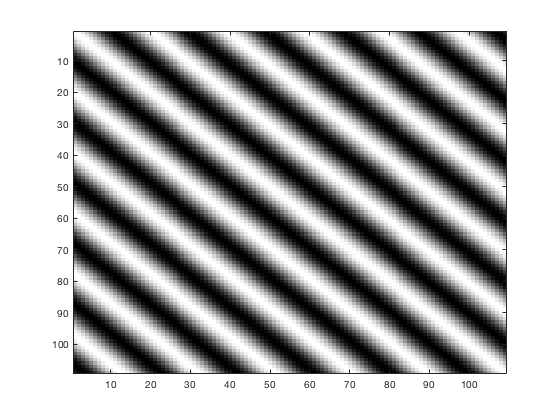
\includegraphics[width=0.6\textwidth]{images/sin2.png}
    \caption{Échantillonnage de $s_{\theta}(t,u)$,
    avec $A=10$, $\theta=45^\circ$, $L=512$, $T_0=64$, et $T_e=\frac{1}{16 \cdot
    f_m}$
}
    \label{img:sin16}
\end{figure}

\textbf{(2b)} Les figures \ref{subimg:ft-sin16-2d} et \ref{subimg:ft-sin16-3d}
contiennent respectivement les spectre 2d et 3d de la Transformée de Fourier
Discrète de l'image précédente.

\begin{figure}[H]
    \centering
    \begin{subfigure}[c]{0.46\textwidth}
        \centering
        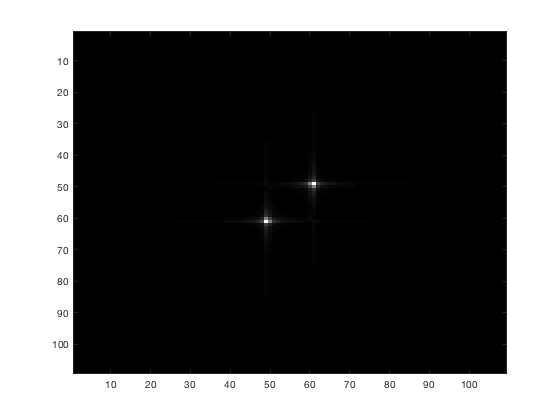
\includegraphics[width=\textwidth]{images/ft1.png}
        \caption{Représentation 2d} 
    \label{subimg:ft-sin16-2d}
    \end{subfigure}
    \begin{subfigure}[c]{0.46\textwidth}
        \centering
        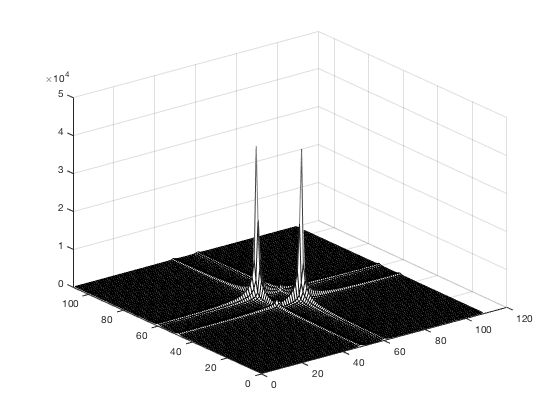
\includegraphics[width=\textwidth]{images/ft13D.png}
        \caption{Représentation 3d}
    \label{subimg:ft-sin16-3d}
    \end{subfigure}
    \label{fig:ft-sin16}
    \caption{Spectres 2d et 3d de la Transformée de Fourier Discrète de
    l'image de la \figref{img:sin16}}
\end{figure}

\textbf{(2c)} On remarque bien la présence de deux pics en fréquence (deux Dirac) sur
les deux figures précédentes. \\

On fait maintenant varier la période d'échantillonnage de la sinusoïde. Les
figures \ref{subimg:ft-5-2D}, \ref{subimg:ft-5-3D} et \ref{subimg:ft-2-2D},
\ref{subimg:ft-2-3D} contiennent respectivement les spectres des signaux produits
avec $T_e = \frac{1}{5 \cdot f_m}$ et $T_e = \frac{1}{2 \cdot f_m}$.

\begin{figure}[H]
    \centering
    \begin{subfigure}[c]{0.46\textwidth}
        \centering
        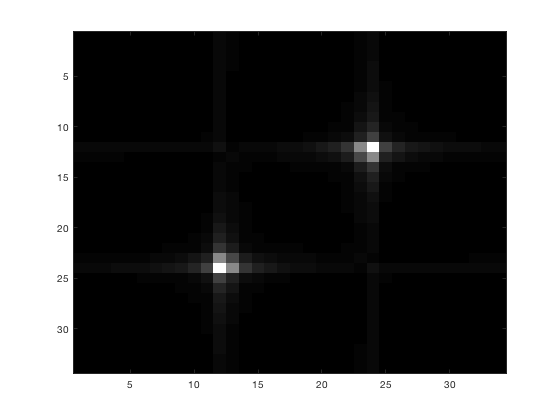
\includegraphics[width=\textwidth]{images/ft2.png}
        \caption{Représentation 2d du spectre de $s_{\theta}(t,u)$, avec $T_e=\frac{1}{5 \cdot f_m}$}
    \label{subimg:ft-5-2D}
    \end{subfigure}
    \begin{subfigure}[c]{0.46\textwidth}
        \centering
        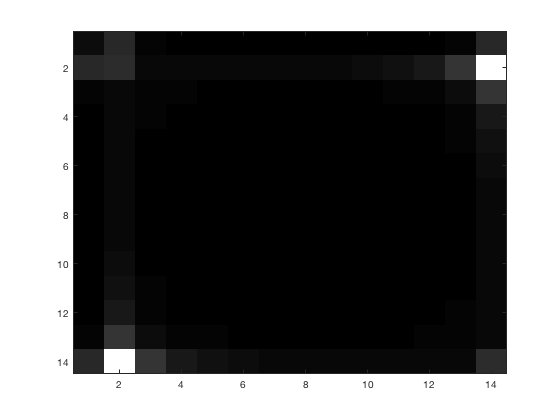
\includegraphics[width=\textwidth]{images/ft3.png}
        \caption{Représentation 2d du spectre de $s_{\theta}(t,u)$, avec $T_e=\frac{1}{2 \cdot f_m}$}
    \label{subimg:ft-2-2D}
    \end{subfigure}
    \begin{subfigure}[c]{0.46\textwidth}
        \centering
        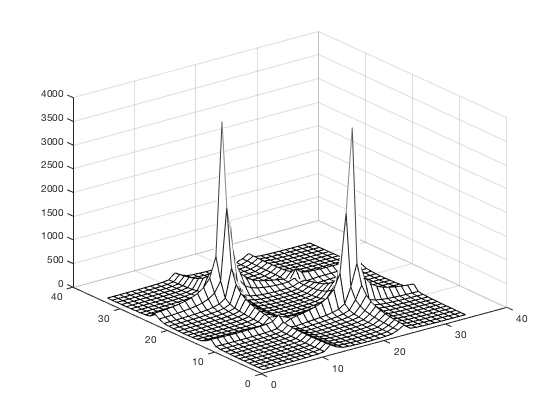
\includegraphics[width=\textwidth]{images/ft23D.png}
        \caption{Représentation 3d du spectre de $s_{\theta}(t,u)$, avec $T_e=\frac{1}{5 \cdot f_m}$}
    \label{subimg:ft-5-3D}
    \end{subfigure}
    \begin{subfigure}[c]{0.46\textwidth}
        \centering
        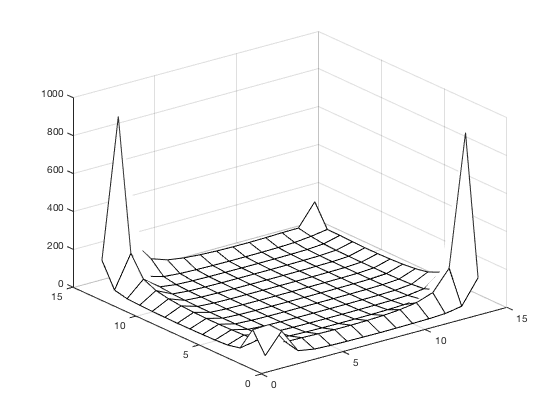
\includegraphics[width=\textwidth]{images/ft33D.png}
        \caption{Représentation 3d du spectre de $s_{\theta}(t,u)$, avec $T_e=\frac{1}{2 \cdot f_m}$}
    \label{subimg:ft-2-3D}
    \end{subfigure}

    \label{img:sin-var}
\end{figure}

D'après l'\eqref{eq:spectre-e}, la période d'échantillonnage $T_e$ intervient
dans la Transformée de Fourier du signal échantillonné. Comme l'on a fait varier
$T_e$, on observe des différences sur le spectre.

Plus la fréquence d'échantillonnage $f_e$ diminue, moins les pics sont distincts
et moins l'image échantillonnée est détaillée.
Lorsque l'on atteint sa valeur limite selon le théorème de Shannon ($f_e = 2$),
on remarque que les pics sont sur les bords. 

\subsection*{Question 3}

On échantillonne maintenant $s_{\theta}(t,u)$ avec $f_e = 4 \cdot f_m$, puis
l'on reconstruit le signal à l'aide de la fonction
\texttt{shannon\_interpolation}, avant de calculer avec \texttt{erreur} l'erreur
moyenne relative de reconstruction.

\begin{figure}[H]
    \centering
    \begin{subfigure}[c]{0.46\textwidth}
        \centering
        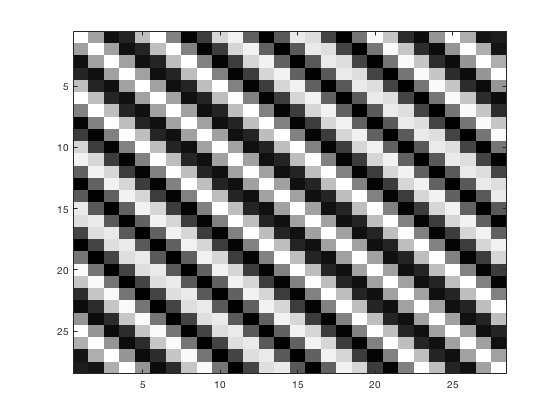
\includegraphics[width=\textwidth]{images/sin-e5.png}
        \caption{Échantillonage de $s_{\theta}(t,u)$, avec $T_e= 4 \cdot f_m$}
    \label{subimg:sin-4-e}
    \end{subfigure}
    \begin{subfigure}[c]{0.46\textwidth}
        \centering
        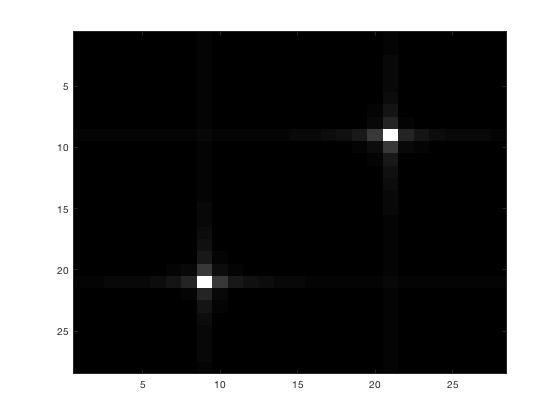
\includegraphics[width=\textwidth]{images/ft52D.png}
        \caption{Représentation 2d du spectre correspondant}
    \label{subimg:ft-4-2D}
    \end{subfigure}
    \begin{subfigure}[c]{0.46\textwidth}
        \centering
        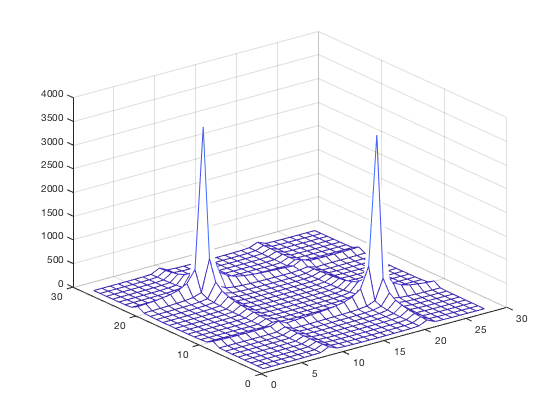
\includegraphics[width=\textwidth]{images/ft53D.png}
        \caption{Représentation 3d du spectre correspondant}
    \label{subimg:ft-4-3D}
    \end{subfigure}
    \begin{subfigure}[c]{0.46\textwidth}
        \centering
        
\includegraphics[width=\textwidth]{images/sin-r5.png}
        \caption{Reconstruction de l'image}
    \label{subimg:sin-4-r}
    \end{subfigure}
    \label{img:sin-4-reconstr}
    \caption{Reconstruction de $s_{\theta}(t,u)$, avec $T_e = 4 \cdot
    f_m$}
\end{figure}

On remarque sur la \figref{subimg:sin-4-r} que les bandes sont légèrement
ondulées. Cette erreur de reconstruction s'explique par une fréquence
d'échantillonnage $f_e$ relativement faible par rapport à la fréquence maximale
$f_m$. Malgré le respect du théorème de Nyquist-Shannon, il y a perte
d'information et l'on ne peut pas reconstruire le signal de façon précise.

\subsection*{Question 4}
On reprend la question 3 avec $f_e = \frac{3}{2} f_{max}$.

\begin{figure}[H]
    \centering
    \begin{subfigure}[c]{0.46\textwidth}
        \centering
        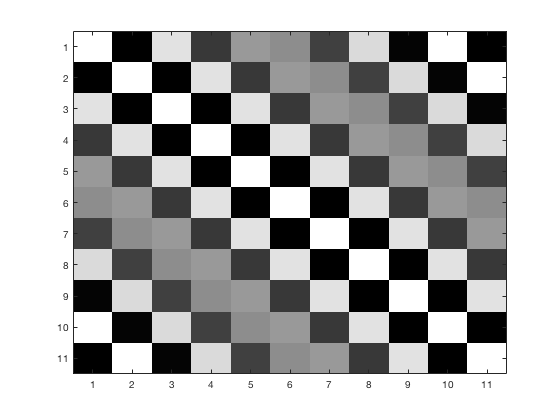
\includegraphics[width=\textwidth]{images/sin-e4.png}
        \caption{Échantillonage de $s_{\theta}(t,u)$, avec $T_e= \frac{3}{2}
        \cdot f_m$}
    \label{subimg:sin-3demi-e}
    \end{subfigure}
    \begin{subfigure}[c]{0.46\textwidth}
        \centering
        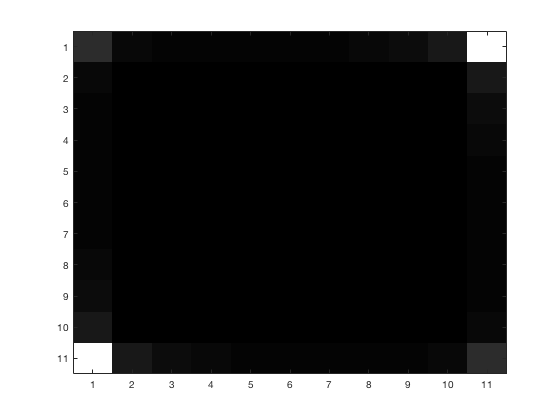
\includegraphics[width=\textwidth]{images/ft42D.png}
        \caption{Représentation 2d du spectre correspondant}
    \label{subimg:ft-3demi-2D}
    \end{subfigure}
    \begin{subfigure}[c]{0.46\textwidth}
        \centering
        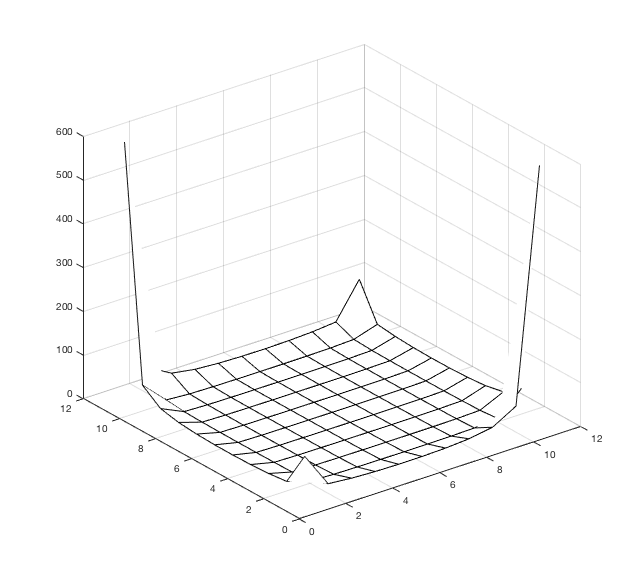
\includegraphics[width=\textwidth]{images/ft43D.png}
        \caption{Représentation 3d du spectre correspondant}
    \label{subimg:ft-3demi-3D}
    \end{subfigure}
    \begin{subfigure}[c]{0.46\textwidth}
        \centering
        
\includegraphics[width=\textwidth]{images/sin-r4.png}
        \caption{Reconstruction de l'image}
    \label{subimg:sin-3demi-r}
    \end{subfigure}
    \label{img:sin-reconstr-3demi}
    \caption{Reconstruction de $s_{\theta}(t,u)$, avec $T_e = \frac{3}{2} \cdot
    f_m$}
\end{figure}

La \figref{subimg:sin-3demi-r} montre un problème de reconstruction de la
sinusoïde : les bandes ne sont pas assez droites. Ce problème est confirmé par
les figures \ref{subimg:sin-3demi-e}, \ref{subimg:ft-3demi-2D}, et
\ref{subimg:ft-3demi-3D}. Comme l'on n'a pas respecté le
théorème de Shannon, on perd trop d'information.

\end{document}
